%% figures/fig5_rk_boundary.tex
%% Fig.5 — K값과 R 경계 시각화 (드래프터별, 워크로드별), 1컬럼

\begin{figure}[t]
\centering
\resizebox{0.95\columnwidth}{!}{%
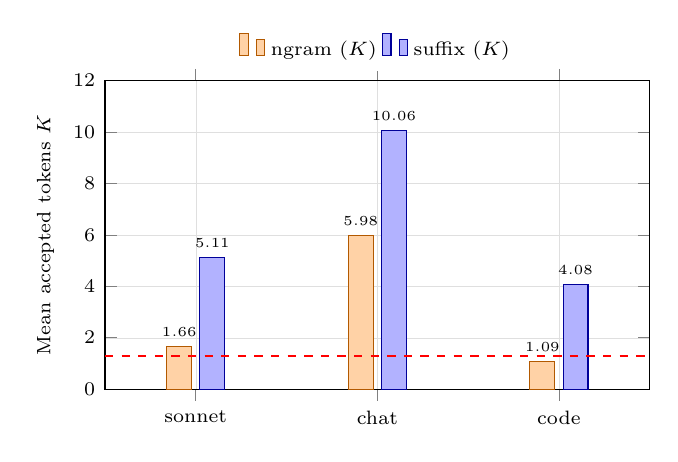
\begin{tikzpicture}
\begin{axis}[
    ybar=3pt,
    bar width=9pt,
    width=8.5cm, height=5.5cm,
    ylabel={Mean accepted tokens $K$},
    ylabel style={font=\scriptsize},
    symbolic x coords={sonnet, chat, code},
    xtick=data,
    xticklabel style={font=\scriptsize},
    yticklabel style={font=\scriptsize},
    ymin=0, ymax=12,
    ytick={0,2,4,6,8,10,12},
    legend style={at={(0.5,1.03)}, anchor=south, legend columns=2,
                  font=\scriptsize, draw=none},
    nodes near coords,
    nodes near coords style={font=\tiny},
    enlarge x limits=0.25,
    grid=major,
    grid style={line width=0.1pt, draw=gray!25},
]
%% ngram K
\addplot[fill=orange!35, draw=orange!70!black] coordinates {
    (sonnet,1.66) (chat,5.98) (code,1.09)};
%% suffix K
\addplot[fill=blue!30, draw=blue!60!black] coordinates {
    (sonnet,5.11) (chat,10.06) (code,4.08)};
%% R threshold line
\draw[red, thick, dashed]
    ({rel axis cs:0,0} |- {axis cs:sonnet,1.3}) --
    ({rel axis cs:1,0} |- {axis cs:sonnet,1.3})
    node[right, font=\tiny, red] {$R \approx 1.3$};
\legend{ngram ($K$), suffix ($K$)}
\end{axis}
\end{tikzpicture}%
}
\caption{드래프터별 평균 수락 토큰 수 $K$ (Llama-3.3-70B, SUB\_093).
  붉은 점선 $R \approx 1.3$은 net-gain 임계값.
  ngram은 code에서 $K=1.09 < R$ → $-20.2\%$ regression.
  suffix는 전 워크로드에서 $K > R$, code에서 suffix/ngram $K$ 비율 $3.74\times$.}
\label{fig:rk-boundary}
\end{figure}
